% la-03-complex.tex

\documentclass[xcolor=dvipsnames]{beamer}
\usepackage{teachbeamer}

\title{Complex Numbers}
\subtitle{{\CourseNumber}, BCIT}

\author{\CourseName}

\date{September 24, 2018}

\begin{document}

\begin{frame}
  \titlepage
\end{frame}

\begin{frame}
  \frametitle{Vector Space}
  A \alert{vector space} $V$ over a field $F$ is a set on which two
  operations (addition and scalar multiplication) are defined. Some
  axioms need to be fulfilled, most relevantly \alert{closure} with
  respect to addition and scalar multiplication:
  \begin{itemize}
  \item If $v,w\in{}V$, then $v+w\in{}V$
  \item If $a\in{}F,v\in{}V$, then $av\in{}V$
  \end{itemize}
  In this course, the field will always be $\mathbb{R}$ or
  $\mathbb{C}$, the real or the complex numbers.
\end{frame}

\begin{frame}
  \frametitle{Complex Numbers}
  The following set
  \begin{equation}
    \label{eq:oiphaebo}
    \mathbb{C}=\{a+bi|a,b\in\mathbb{R}\}
  \end{equation}
  is called the set of complex numbers. Note that
  $\mathbb{R}\subset\mathbb{C}$. Operations (addition, multiplication,
  and so on) are defined on complex numbers the same way as on real
  numbers with one additional rule:
  \begin{equation}
    \label{eq:thaikiec}
    i^{2}=-1
  \end{equation}
\end{frame}

\begin{frame}
  \frametitle{Complex Operators}
  {\ubung} Find the determinant of the following matrix:
  \begin{equation}
    \label{eq:ohhohhoo}
    A=\left[
      \begin{array}{cc}
        1-4i & 3-i \\
        -3i & 3+4i
      \end{array}\right]
  \end{equation}
{\ubung} A matrix that equals its conjugate transpose is called a
\alert{Hermitian matrix}. Calculate the determinate of the following
example.
\begin{equation}
  \label{eq:ohsaiphi}
  B=\left[
    \begin{array}{ccc}
      2 & 2+i & 4 \\
      2-i & 3 & i \\
      4 & -i & 1
    \end{array}\right]
\end{equation}
{\ubung} Use expansion by conjugates to divide
\begin{equation}
  \label{eq:choomeux}
  \frac{7-2i}{3+4i}
\end{equation}
\end{frame}

\begin{frame}
  \frametitle{Polar Form}
  The complex numbers correspond to vectors in $\mathbb{R}^{2}$.
    \begin{figure}[h]
    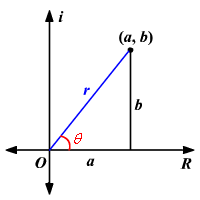
\includegraphics[scale=0.32]{./diagrams/polar.png}
  \end{figure}
Instead of providing the coordinates $(a,b)$ of a complex number, it
is sometimes useful to provide the \alert{polar form} $(r,\theta)$.
\begin{equation}
  \label{eq:eekaerai}
  \begin{array}{ll}
    a=r\cos\theta & b=r\sin\theta \\
    r^{2}=a^{2}+b^{2} & \tan\theta=\frac{b}{a}
  \end{array}
\end{equation}
A complex number $a+bi$ can always be written in its polar form $a+bi=r(\cos\theta+i\sin\theta)$.
\end{frame}

\begin{frame}
  \frametitle{Euler's Formula}
  One of the most famous formulas in mathematics is Euler's formula
  \begin{equation}
    \label{eq:kiagaiga}
    e^{ix}=\cos{}x+i\sin{}x
  \end{equation}
For the proof, we need some calculus. Recall the Maclaurin series
expansions
\begin{equation}
  \label{eq:uthairoj}
  e^{x}=\sum_{j=0}^{\infty}\frac{x^{j}}{j!}
\end{equation}
\begin{equation}
  \label{eq:eepiewez}
  \cos{}x=\sum_{j=0}^{\infty}(-1)^{j}\frac{x^{2j}}{(2j)!}
\end{equation}
\begin{equation}
  \label{eq:mohhaich}
  \sin{}x=\sum_{j=0}^{\infty}(-1)^{j}\frac{x^{2j+1}}{(2j+1)!}
\end{equation}
Calculus still works in the complex numbers, now try to find $e^{ix}$. 
\end{frame}

\begin{frame}
  \frametitle{Use of the Polar Form}
Euler's formula makes multiplication, division, exponentiation and
finding roots of complex numbers in polar form more simple.

\medskip

{\ubung} Multiply $(4,60^{\circ})$ by $(2,20^{\circ})$, where the
given factors are complex numbers provided in polar form.

\medskip

{\ubung} Divide $(8,100^{\circ})$ by $(4,65^{\circ})$, where the
given numbers are complex numbers provided in polar form.

\medskip

{\ubung} Find, using two alternative ways,
\begin{equation}
  \label{eq:iekaekep}
  \frac{-2+5i}{-1-i}\mbox{ and }\left(2+3i\right)^{5}
\end{equation}
\end{frame}

\begin{frame}
  \frametitle{Closeted Functions}
You may remember that I once called trigonometric functions ``closeted
exponential functions.'' Here is the reason. Consider
\begin{equation}
  \label{eq:eixeivei}
  \begin{array}{rcl}
  e^{ix}&=&\cos{}x+i\sin{}x \\
  e^{-ix}&=&\cos{}x-i\sin{}x
  \end{array}
\end{equation}
Add and subtract these two equations for
\begin{equation}
  \label{eq:ohrayaxu}
  \cos{}x=\frac{e^{ix}+e^{-ix}}{2}
\end{equation}
\begin{equation}
  \label{eq:quuiquei}
  \sin{}x=\frac{e^{ix}-e^{-ix}}{2i}
\end{equation}
This is the definition of trigonometric functions on $\mathbb{C}$. The
hyperbolic trigonometric functions are closeted sines and cosines,
since $\cosh(x)=\cos(ix)$ and $i\sinh(x)=\sin(ix)$. 
\end{frame}

\begin{frame}
  \frametitle{de Moivre's Formula}
\begin{block}{de Moivre's Formula}
  $\left(re^{i\theta}\right)^{n}=r^{n}e^{in\theta}$
\end{block}

\medskip

\beispiel{Cube Roots} Find the solution set for the following equation
and $c=(27,120^{\circ})$, where $c$ is a complex number provided in
polar form.
\begin{equation}
  \label{eq:aephacha}
  x^{3}=c
\end{equation}

\medskip

By de Moivre's formula, $x=(3,40^{\circ})$ is a solution. However,
$c=(27,480^{\circ})$ and therefore, by de Moivre's formula again,
$x=(3,160^{\circ})$ is also a solution. $c=(27,840^{\circ})$ provides
the third solution, $x=(3,280^{\circ})$. Polynomial equations of
degree $n$ usually have $n$ solutions in $\mathbb{C}$. 
\end{frame}

\begin{frame}
  \frametitle{Exponents and Square Roots}
  \beispiel{Real Exponent} Find $x=(2-3i)^{3}$. Expanding the product
  gives us $-46-9i$. If we convert to polar form,
  \begin{equation}
    \label{eq:akingahg}
    \left(\sqrt{13}\left(\cos(-56.31^{\circ})+i\sin(-56.31^{\circ})\right)\right)^{3}=\notag
  \end{equation}
  \begin{equation}
    \label{eq:ohsegeel}
    \left(\sqrt{13}\left(e^{i\cdot{}(-56.31^{\circ})}\right)\right)^{3}=13^{\frac{3}{4}}\left(\cos(-168.93^{\circ})+i\sin(-168.93^{\circ})\right)=\notag
  \end{equation}
  \begin{equation}
    \label{eq:ciesoola}
  -46-9i\notag
  \end{equation}
\end{frame}

\begin{frame}
  \frametitle{Exponents and Square Roots}
  \beispiel{Square Root} Find $\sqrt{2-3i}$. Converting to polar form,
  \begin{equation}
    \label{eq:etahmohy}
    \left(\sqrt{13}\left(\cos(-56.31^{\circ})+i\sin(-56.31^{\circ})\right)\right)^{\frac{1}{2}}=\notag
  \end{equation}
  \begin{equation}
    \label{eq:thueceij}
    \left(\sqrt{13}\left(e^{i\cdot{}(\alert{-56.31^{\circ}})}\right)\right)^{\frac{1}{2}}=13^{\frac{1}{4}}\left(\cos(-28.55^{\circ})+i\sin(-28.55^{\circ})\right)\approx\notag
  \end{equation}
  \begin{equation}
    \label{eq:puxiengo}
    1.6741-0.89598i\notag
  \end{equation}
  However, notice that the last two lines could also be
  \begin{equation}
    \label{eq:guwohdoh}
    \left(\sqrt{13}\left(e^{i\cdot{}(\alert{303.69^{\circ}})}\right)\right)^{\frac{1}{2}}=13^{\frac{1}{4}}\left(\cos(151.85^{\circ})+i\sin(151.85^{\circ})\right)\approx\notag
  \end{equation}
  \begin{equation}
    \label{eq:jahwiebo}
    -1.6741+0.89598i\notag
  \end{equation}
  which is clearly a different number.
\end{frame}

\begin{frame}
  \frametitle{Complex Roots}
  \beispiel{Cube Roots of 27} One is easy to find: the number 3,
  multiplied by itself three times, gives us 27. Where are the other
  two cube roots of 27? Consider
\begin{equation}
  \label{eq:eecohghu}
  27^{\frac{1}{3}}=(27+0i)^{\frac{1}{3}}=\left(27(\cos{})^{\circ}+i\sin{}0^{\circ})\right)^{\frac{1}{3}}\notag
\end{equation}
\begin{equation}
  \label{eq:vuphahdo}
  \overset{(1)}{=}\left(27^{\frac{1}{3}}\left(e^{\frac{1}{3}i\cdot{}\alert{0^{\circ}}}\right)\right)=3e^{i\cdot{}\alert{0^{\circ}}}=3\notag
\end{equation}
\begin{equation}
  \label{eq:yudiesoo}
  \overset{(2)}{=}\left(27^{\frac{1}{3}}\left(e^{\frac{1}{3}i\cdot{}\alert{360^{\circ}}}\right)\right)=3e^{i\cdot{}\alert{120^{\circ}}}=-1.5+1.5\sqrt{3}\cdot{}i\notag
\end{equation}
\begin{equation}
  \label{eq:vaimetha}
  \overset{(3)}{=}\left(27^{\frac{1}{3}}\left(e^{\frac{1}{3}i\cdot{}\alert{720^{\circ}}}\right)\right)=3e^{i\cdot{}\alert{240^{\circ}}}=-1.5-1.5\sqrt{3}\cdot{}i\notag
\end{equation}
\end{frame}

\begin{frame}
  \frametitle{Fundamental Theorem of Algebra}
    \begin{figure}[h]
    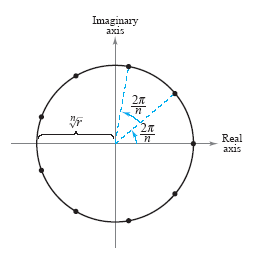
\includegraphics[scale=0.65]{./diagrams/comproot.png}
  \end{figure}
\end{frame}

\begin{frame}
  \frametitle{Fundamental Theorem of Algebra}
  {\ubung} Solve the equation
  \begin{equation}
    \label{eq:phoojahs}
    x^{2}+4x+5=0
  \end{equation}
  in the complex numbers.
  \begin{block}{Fundamental Theorem of Algebra}
    Every non-constant polynomial equation with complex coefficients
    has a complex solution (usually the number of solutions equals the
    degree of the polynomial). $\mathbb{C}$ is algebraically closed,
    while $\mathbb{R}$ is not.
  \end{block}
\end{frame}

\begin{frame}
  \frametitle{Casus Irreducibilis}
  What is the use of complex numbers? There are many engineering
  examples, but here is one from solving cubic equations. Find the
  solutions for
  \begin{equation}
    \label{eq:oozaechi}
    x^{3}-3x+1=0
  \end{equation}
  Cardano's formula gives us the three solutions,
  \begin{equation}
    \label{eq:iejopice}
    x_{k}=w_{k}\sqrt[3]{-\frac{1}{2}+\sqrt{\frac{-3}{4}}}+w_{k}^{2}\sqrt[3]{-\frac{1}{2}-\sqrt{\frac{-3}{4}}}
  \end{equation}
  where $k=1,2,3$ and $(w_{1},w_{2},w_{3})$ are the three cube roots
  of $1$. You can look up online why Cardano's formula is true. The
  point is that all the solutions to this problem are real numbers,
  but we have to use complex algebra to calculate them.
\end{frame}

\begin{frame}
  \frametitle{End of Lesson}
Next Lesson: Vector Spaces
\end{frame}

\end{document}

